\chapter{Derivadas}
A \emph{derivada} de uma função $f$ em um ponto $x$ é o coeficiente angular da reta tangente ao gráfico desta função no ponto $(x, f(x))$.\par Para determinarmos a reta tangente, definimos uma reta secante à função, como a reta em vermelho no gráfico abaixo. A partir da reta secante, reduzimos a \emph{distância incremental} $h$, aproximando os pontos $(x,f(x))$ e $(x+h,f(x+h))$. \par 
Como não podemos definir uma reta por apenas um ponto, tomamos o limite de $h \rightarrow 0$, aproximando os pontos ao máximo.

\begin{figure}[H]
	\centering
		\begin{tikzpicture}
		\begin{axis}[
		axis lines = middle,
        ytick = {0.48168,0.73146},
        yticklabels = {$f(x)$,$f(x+h)$},
        xtick = {0.13814,0.49277},
        xticklabels = {$x$,$x+h$},
        ymin = 0,
        restrict y to domain = 0:2,
        ymax = 1, 
		xmin = 0,
        xmax = 1,
        xlabel = $x$,
        ylabel = $y$]
        \addplot[
        domain = 0:2,
        samples = 100,
        ]{((4*(x+0.033)-1.126)^7)/3.5+0.01*(x-1.09)+0.49};
        \addplot[ %secante
        domain = 0:2,
        samples = 3,
        olive!40!lime,
        thick,
        ]{0.704*x+0.3843};
        \addplot[
        domain = 0:0.13814,
        samples = 100,
        dashed
        ]{0.48168};
        \addplot[  %ponto (x+h,f(x+h))
        domain = 0:0.49277,
        samples = 3,
        dashed
        ]{0.73146};
        \addplot[
        dashed,
        samples=3, 
        domain=0:6,
        ] coordinates {(0.49277,0)(0.49277,0.73146)};        
        \addplot[ %ponto (x, f(x))
        domain = 0:0.13814,
        samples = 3,
        dashed
        ]{0.48168};
        \addplot[
        dashed,
        samples=3, 
        domain=0:6,
        ] coordinates {(0.13814,0)(0.13814,0.48168)};
		\end{axis}
        \end{tikzpicture}
\end{figure}

\begin{df}
Sejam $f$ uma função. A \emph{derivada} da função $f$ é chamada $f'$ e definida por
\[f'(x)=\displaystyle\lim_{h\rightarrow 0}\dfrac{f(x+h)-f(x)}{h}\] desde que exista o limite. \\
A \emph{reta tangente} à curva $f$ em $(a,f(a))$ é a reta que passa por $(a,f(a))$ e tem coeficiente angular $f'(a)$.
\end{df}
A equação da reta tangente em um ponto $x=p$ é dada por $(y-y_p)=f'(p)(x-x_p)$.

\begin{exemplo}
Dada $f(x)=x^2$, determine a reta tangente a $f$ no ponto de $x=2$. \par 
Para isso, iremos utilizar a definição de derivada:
\begin{align*}
\lim_{h\rightarrow0}\dfrac{(2+h)^2-(2)^2}{h} &= \lim_{h\rightarrow0}\dfrac{(4+4h+h^2)-(4)}{h} \\
&= \lim_{h\rightarrow0}\dfrac{(4h+h^2)}{h} \\
&= \lim_{h\rightarrow0}\dfrac{4+h}{1} \\
f'(2)&= 4
\end{align*}
Para encontrarmos a equação da reta tangente, usaremos $f(2)=2^2=4$. Assim, temos:
\begin{align*}
(y-y_p)&=f'(p)(x-x_p) \\
y-4&=4(x-2) \\
y-4 &=4x-8 \\
y &= 4x-4
\end{align*}
Dada $g(x)=\frac{1}{x}$, determine a inclinação reta tangente no ponto $x=2$. \par 
Novamente, utilizaremos a definição:
\begin{align*}
\lim_{h\rightarrow0}\dfrac{\frac{1}{2+h}-\frac{1}{2}}{h}=&\lim_{h\rightarrow0}\dfrac{1}{h}\cdot\dfrac{2-(2+h)}{2(2+h)} \\
=&\lim_{h\rightarrow0}\dfrac{-h}{2h(2+h)} \\
=&\lim_{h\rightarrow0}\dfrac{-1}{2(2+h)} \\
=&\lim_{h\rightarrow0}\dfrac{-1}{4+2h} \\
g'(2)=&\dfrac{-1}{4}
\end{align*}
\end{exemplo} \par 
Podemos, também, visualizar a derivada como uma função.
\begin{exemplo}
Determine a função $f'(x)$ que fornece o coeficiente angular da reta tangente aos pontos da função definida por $f(x)=3x^2$. \par
Para isso, basta não atribuirmos valores a $x$.
\begin{align*}
\lim_{h\rightarrow0}\dfrac{3(x+h)^2-3(x)^2}{h}=&\lim_{h\rightarrow0}\dfrac{3(x^2+2xh+h^2)-3x^2}{h} \\
=&\lim_{h\rightarrow0}\dfrac{{3x^2}+6xh+3h^2-{3x^2}}{h} \\
=&\lim_{h\rightarrow0}\dfrac{6xh+3h^2}{h} \\
=&\lim_{h\rightarrow0}\dfrac{6x+h}{1} \\
f'(x)=&6x
\end{align*}
Com a função $f'(x)=6x$, podemos determinar facilmente o coeficiente angular da reta tangente a $f$ para qualquer ponto do domínio de $f$.
\end{exemplo} \par 
Podemos utilizar uma versão equivalente da definição de derivada, que pode facilitar o cálculo:
\[\lim_{z\rightarrow x}\dfrac{f(z)-f(x)}{z-x}\]

\section{Funções Diferenciáveis}
\begin{df}
Uma função $y=f(x)$ será \emph{diferenciável} em um intervalo aberto (finito ou infinito) se tiver uma derivada em cada ponto do intervalo. Será diferenciável em um intervalo fechado $[a,b]$ se for diferenciável no intervalo $(a,b)$ e se os limites
\[\lim_{h\rightarrow 0^+}\dfrac{f(a+h)-f(a)}{h} \qquad \textbf{Derivada à direita em a}\]
\[\lim_{h\rightarrow 0^-}\dfrac{f(b+h)-f(b)}{h} \qquad \textbf{Derivada à esquerda em b}\]
existirem nas extremidades do intervalo.
\end{df} \par
As derivadas à direita e à esquerda podem ser definidas em qualquer ponto do domínio, mas são especialmente interessantes para determinar se a função é diferenciável em um intervalo fechado. Por isso, não iremos trabalhar com exemplos de derivadas laterais. \par 
Resumindo a definição, temos que funções são diferenciáveis no domínio de sua derivada.
\subsection{Pontos não-diferenciáveis}
Uma função possui derivada quando possui o limite do coeficiente angular da reta tangente. Quando as retas secantes não apresentam um limite (que resultaria na derivada) ou se tornam verticais a medida que $h \rightarrow 0$, a derivada não existe. Assim, a diferenciabilidade de uma função depende da ``suavidade'' do gráfico da função.
\paragraph{Bico} Ponto contínuo do domínio onde as derivadas laterais são diferentes.
\paragraph{Ponto Cuspidal} Onde o coeficiente angular tende a $\infty$ por um lado e $-\infty$ por outro.
\paragraph{Tangente Vertical} Onde o coeficiente angular tende a $\infty$ (ou $-\infty$) por ambos os lados.
\paragraph{Descontinuidade} A função apresenta uma descontinuidade no ponto.

\begin{teo}\marginnote{Devemos tomar cuidado com a recíproca deste teorema. Nem toda função contínua em um intervalo é diferenciável neste intervalo. Por exemplo, $f(x)=\sqrt[3]{x^2}$, contínua em $\mathbb{R}$, cuja derivada $f'(x)=\frac{2}{3\sqrt[3]{x}}$ não existe no ponto $x=0$).}
Se $f$ tem uma derivada em $x=c$, então $f$ é contínua em $x=c$.
\begin{proof}
Como $f'(c)$ existe, devemos mostrar que $\lim_{x\rightarrow c}f(x)=c$ ou, de maneira equivalente, que $\lim_{h\rightarrow 0}f(c+h)=f(c)$. Se $h\neq0$, então
\begin{align*}
f(c+h)=&f(c)+(f(c+h)-f(c))\\
=&f(c)+\dfrac{\left[f(c+h)-f(c)\right]}{h}\cdot h
\end{align*}
Agora, tomando o limite quando $h \rightarrow 0 $, temos
\begin{align*}
\lim_{h\rightarrow0}f(c+h)=&\lim_{h\rightarrow0}f(c)+\lim_{h\rightarrow0}\dfrac{f(c+h)-f(c)}{h}\cdot \lim_{h\rightarrow0}h \\
=&f(c)+f'(c)\cdot0\\
=&f(c)
\end{align*}
Assim, se uma função possui derivada em um ponto, a função é contínua no ponto.
\end{proof}
\end{teo}

\section{Regras de Derivação}
Para evitar a aplicação da definição em derivadas, foram desenvolvidas certas regras para tornar o processo mais rápido. Estas regras permitem derivar uma grande variedade de funções, como as polinomiais, trigonométricas, produtos e quocientes. Além disso, todas as regras aqui apresentadas podem ser demonstradas a partir da definição. \par Utilizaremos $c$ como uma constante qualquer e $u,v$ como funções de $x$ para evitar confusão com $f$ e $g$.

\subsection{Polinomiais}
\begin{align*}
\dfrac{d}{dx}(c)&=0 \\ \dfrac{d(x)}{dx}&=1 \\ \dfrac{d}{dx}(x^n)&=nx^{n-1}, \: \forall n \neq 0 \\ \dfrac{d}{dx}\left(c\cdot u\right)&=c\cdot \left(\dfrac{du}{dx}\right) \\ \dfrac{d}{dx}(u\pm v)&=\dfrac{du}{dx}\pm \dfrac{dv}{dx} \\ 
\end{align*}
\begin{exemplo}
\begin{align*}
f(x)=3x^2+10 \Rightarrow \dfrac{df}{dx}&=\dfrac{d}{dx}(3x^2+10)\\ &=\dfrac{d}{dx}(3x^2)+\dfrac{d}{dx}(10) \\ &=3\dfrac{d}{dx}(x^2)+0 \\ &=3\cdot 2x^{2-1}\\ &=6x
\end{align*}
\begin{align*}
\dfrac{d(\sqrt[3]{x})}{dx}&=\dfrac{d(x^{\frac{1}{3}})}{dx}\\
&=\dfrac{1}{3}x^{\frac{1}{3}-1}\\
&=\dfrac{x^{-\frac{2}{3}}}{3}\\
&=\dfrac{1}{3\sqrt[3]{x^2}}
\end{align*}
\end{exemplo}

\subsection{Produto e Quociente}
\begin{align*}
\dfrac{d}{dx}(uv)&=u\dfrac{dv}{dx}+v\dfrac{du}{dx}\\
\dfrac{d}{dx}\left(\dfrac{u}{v}\right)&=\dfrac{v\frac{du}{dx}-u\frac{dv}{dx}}{v^2}
\end{align*}
\begin{exemplo}
\begin{align*}
g(x)&=(3x^2-5)(x^3+2x) \\ \dfrac{dg}{dx} &=\dfrac{d}{dx}(3x^2-5)\cdot (x^3+2x) + \dfrac{d}{dx}(x^3+2x) \cdot (3x^2-5) \\
&=(6x)(x^3+2x)+(3x^2+2)(3x^2-5) \\
&= 6x^4+12x^2+9x^4-15x^2+6x^2-10 \\
&= 15x^4+3x^2-10
\end{align*}
\begin{align*}
f(x)=\dfrac{3x}{x^2+1} \Rightarrow \dfrac{df}{dx}&=\dfrac{d}{dx}\left(\dfrac{3x}{x^2+1}\right)\\
&=\dfrac{(x^2+1)\cdot\frac{d}{dx}(3x)-3x\cdot\frac{d}{dx}(x^2+1)}{(x^2+1)^2}\\
&=\dfrac{3\cdot(x^2+1)-3x\cdot(2x)}{(x^2+1)^2} \\
&=\dfrac{3x^2+3-6x^2}{(x^2+1)^2} \\
&=\dfrac{-3x^2+3}{(x^2+1)^2}
\end{align*}
Tomemos a função $y=1/x$. Repare que podemos resolvê-la de duas formas, obtendo o mesmo resultado:
\begin{align*}
\dfrac{dy}{dx}&=\dfrac{d(x^{-1})}{dx}\\ &=-1\cdot x^{-1-1}=-x^{-2}\\ &=-\dfrac{1}{x^2} \\
\textrm{Ou então:}\\
\dfrac{dy}{dx}&=\dfrac{d}{dx}\left(\dfrac{1}{x}\right)\\
&=\dfrac{(1)'(x)-(x)'(1)}{(x)^2}\\
&=-\dfrac{1}{x^2}
\end{align*}
\end{exemplo}

\subsection{Exponencial e Logarítmica}
\begin{align*}
\dfrac{d}{dx}\log_a x=\dfrac{1}{x\ln(a)} &\Rightarrow \dfrac{d(\ln x)}{dx}=\dfrac{1}{x}\\
\dfrac{d}{dx}(a^x)=a^x \ln(a) &\Rightarrow \dfrac{d(e^x)}{dx}=e^x
\end{align*}
\begin{exemplo}
\begin{align*}
\dfrac{d}{dx}\left(e^x\cdot \ln(x)\right)&=(e^x)'\ln(x) + \left(\ln(x)\right)'e^x\\
&=e^x\ln(x)+\frac{e^x}{x}=e^x\left(\ln(x)+\frac{1}{x}\right)
\end{align*}
\begin{align*}
\dfrac{d}{dx}(xe^x)&=\dfrac{dx}{dx}e^x+\dfrac{d(e^x)}{dx}x\\
&=e^x+x e^x\\
&=e^x(x+1)
\end{align*}
\end{exemplo}

\subsection{Trigonométricas}
\begin{align*}
 \marginnote{Repare que todas as derivadas de funções trigonométricas que iniciam com ``co'' possuem o sinal negativo e ``co'' nas funções trigonométricas da derivada (exceto o cosseno).} \dfrac{d(\sin (x))}{dx}&=\cos(x) \\
\dfrac{d(\cos(x))}{dx}&=-\sin(x) \\
\dfrac{d(\tan(x))}{dx}&=\sec^2(x) \\
\dfrac{d(\cot(x))}{dx}&=-\csc^2(x) \\
\dfrac{d(\sec(x))}{dx}&=\sec(x)\tan(x) \\
\dfrac{d(\csc(x))}{dx}&=-\csc(x)\cot(x) \\
\end{align*}
\begin{exemplo}
\begin{align*}
\dfrac{d}{dx}\tan(x)&=\dfrac{d}{dx}\left(\dfrac{\sin(x)}{\cos(x)}\right)\\
&=\dfrac{\cos(x)\frac{d(\sin(x))}{dx}-\sin(x)\frac{d(\cos(x))}{dx}}{(\cos(x))^2}\\
&=\dfrac{\cos^2(x)+\sin^2(x)}{\cos^2(x)}\\
&=\dfrac{1}{\cos^2(x)}\\
&=\sec^2(x)
\end{align*}
\end{exemplo}

\section[Regra da Cadeia]{Funções Compostas}
\begin{exemplo}
Seja $y=f(x)=9x^2-6x+1=(3x-1)^2$. Assim, podemos escrever $f(u)=u^2$, sendo $u=3x-1$. Calculando as derivadas de $\dfrac{dy}{dx}$, $\dfrac{dy}{du}$ e $\dfrac{du}{dx}$, temos:
\begin{align*}
\dfrac{dy}{dx}&=18x-6 \\
\dfrac{dy}{du}&=2u \\
\dfrac{du}{dx}&=3 \\
\dfrac{dy}{du}\cdot \dfrac{du}{dx}&=6u=6(3x-1)=18x-6
\end{align*}

Assim, temos que $\dfrac{dy}{dx}=\dfrac{dy}{du}\cdot \dfrac{du}{dx}$.
\end{exemplo}

\begin{teo}[Regra da Cadeia]
Se $f(u)$ é diferenciável no ponto $u=g(x)$ e $g(x)$ é diferenciável em $x$, então a função composta $(f\circ g)(x)=f(g(x))$ é diferenciável em $x$ e \[(f\circ g)'(x)=f'(g(x))\cdot g'(x)\] Na notação de Leibniz, se $y=f(u)$ e $u=g(x)$, então \[\dfrac{dy}{dx}=\dfrac{dy}{du}\cdot \dfrac{du}{dx}\].
\end{teo}

Após desenvolver as regras práticas para a derivação de funções simples, utilizamos a \emph{Regra da Cadeia} para derivar funções compostas, como $y=\sin(x^2)$, onde temos $y=\sin(u)$ e $u=f(x)$. Para isso, devemos considerar a derivada da função interna (neste caso, $x^2$) e a relação com a derivada da externa (neste caso, $\sin(u)$).
\begin{exemplo}
Resolvendo o exemplo acima:
\begin{align*}
y&=\sin(x^2)\\
\dfrac{dy}{dx}&=\dfrac{dy}{du}\cdot \dfrac{du}{dx}\\
&=\cos(x^2)\cdot 2x\\
&=2x\cos(x^2)
\end{align*}
\end{exemplo}

Podemos, também, lembrar da regra da cadeia como ``deriva a de fora, conservando a de dentro, vezes a derivada da de dentro''. Isso facilita para resolver regras da cadeia com mais de duas funções compostas.
\begin{exemplo}
Seja $y=\sin^2(2x+1)$. Assim, temos $y=u^2$, onde $u=\sin(v)$, sendo $v=2x+1$. Aplicando repetidamente a definição, temos:
\[\dfrac{dy}{dx}=\dfrac{dy}{du}\cdot \dfrac{du}{dv} \cdot \dfrac{dv}{dx}\]
Para resolver, realizamos o mesmo procedimento:
\begin{align*}
y &=\sin^2(2x+1) \\
y' &=2\sin(2x+1) \cdot [ \sin(2x+1)]' \\
y' &=2\sin(2x+1) \cdot \cos(2x+1) \cdot (2x+1)' \\
y' &=2\sin(2x+1) \cdot \cos(2x+1) \cdot 2 \\
y' &=4\sin(2x+1) \cos(2x+1)
\end{align*}
\end{exemplo}

\subsection{Derivação Implícita}
A maioria das funções com que lidamos são da forma $y=f(x)$, onde temos explicitamente $y$ em função de $x$. Quando encontramos equações do tipo $F(x,y)=0$, nem sempre podemos escrevê-las na forma $y=f(x)$ para derivá-la de maneia usual. Ainda assim, podemos determinar $dy/dx$ por intermédio da \emph{derivação implícita}. \par Para isso, simplesmente derivamos ambos os lados da equação em relação a $x$, considerando $y=f(x)$ como uma função diferenciável de $x$.
\begin{exemplo}
Seja a equação $y^2=x$. Esta define duas funções diferenciáveis, $y_1=\sqrt{x}$ e $y_2=-\sqrt{x}$. No entanto, podemos determinar $dy/dx$ sem conhecer estas funções:
\begin{align*}
y^2=x\\
\dfrac{d}{dx}(y^2)=\dfrac{dx}{dx}\\
2y\cdot y' =1\\
y'=\dfrac{1}{2y}
\end{align*}

\begin{center}
	\begin{tikzpicture}
		\begin{axis}[
		axis lines = middle,
        ymin = -3,
		ytick = {-2,-1,...,1,2},
        ymax = 3, 
		xmin = 0,
        xmax = 5.5,
        xlabel = $x$,
        ylabel = $y$]
        \addplot[ %curva superior
        domain = 0:8,
        samples = 150,
        ]{sqrt(x)};
        \addplot[ %curva inferior
        domain = 0:8,
        samples=150,
        ]{-sqrt(x)};        
		\end{axis}
	\end{tikzpicture}
\end{center}
Esta fórmula sozinha fornece as derivadas para as funções explícitas $y_1$ e $y_2$.
\end{exemplo}
Podemos determinar $dy/dx$ facilmente por meio destes três passos a seguir:
\begin{enumerate}[1.]
\item Derive os dois lados da equação em realação a $x$, considerando $y=f(x)$ - ou seja, aplicando a regra da cadeia em $y$.
\item Reúna os termos que contêm $y'=dy/dx$ em um lado da equação.
\item Encontre $dy/dx$.
\end{enumerate}
Podemos utilizar $dy/dx$ determinado implicitamente para encontrar a reta tangente a curva e a \emph{reta normal} a esta. A reta normal é a reta perpendicular a reta tangente no ponto de tangência.
\begin{exemplo}
Seja a curva definida implicitamente pela equação $x^3+y^3-9xy=0$. Determinaremos a reta normal a curva no ponto $(2,4)$.
Assim, precisamos do coeficiente angular da reta, dado por $dy/dx$.
\begin{center}
	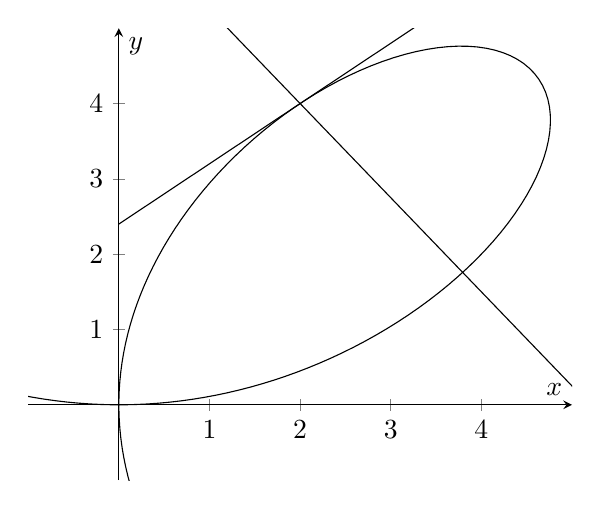
\begin{tikzpicture}
		\begin{axis}[
		axis lines = middle,
        ymin = -1,
		ytick = {0,1,2,3,4},
        ymax = 5, 
		xmin = -1,
        xtick = {0,1,2,3,4},
        xmax = 5,
        xlabel = $x$,
        ylabel = $y$,
        width = 0.7\textwidth]
        \addplot[ %reta tangente
        domain = 0:8,
        samples = 2,
        ]{0.8*x+2.4};
        \draw[samples=200,domain=125:-35]plot(\x:{9*sin(\x)*cos(\x)/(sin(\x)^3+cos(\x)^3)}); % AINDA NÃO
        \addplot[ %reta normal
        domain = 0:8,
        samples = 2,
        ]{-1.25*x+6.5};        
		\end{axis}
	\end{tikzpicture}%
\end{center}%
\begin{align*}
x^3+y^3-9xy&=0 \\
\dfrac{d}{dx}(x^3)+\dfrac{d}{dx}y^3 -9 \dfrac{d}{dx}(xy)&=0 \\
3x^2+3y^2y'-9\cdot \left[x\dfrac{dy}{dx}+y\dfrac{dx}{dx}\right]&=0 \\
3x^2+3y^2y'-9\left(xy'+y\right)&=0\\
3x^2+3y^2y'-9xy'-9y&=0\\
3y^2y'-9xy'&=9y-3x^2 \\
y'=\dfrac{9y-3x^2}{3y^2-9x}&=\dfrac{3y-x^2}{y^2-3x} \\
\end{align*}
A partir desta equação, podemos determinar $dy/dx$:
\begin{align*}
y'&=\dfrac{3(4)-(2)^2}{(4)^2-3(2)} \\
y'&=\dfrac{12-4}{16-6}\\
y'&=\dfrac{8}{10}=\dfrac{4}{5}
\end{align*}
Assim, a reta tangente a curva no ponto $(2,4)$ é:
\begin{align*}
y-(4)&=\dfrac{4}{5}(x-2) \\
y&=\dfrac{4x}{5}-\dfrac{8}{5}+\dfrac{20}{5}\\
y&=\dfrac{4x}{5}+\dfrac{12}{5}
\end{align*}
A reta normal a curva em $(2,4)$ é a reta perpendicular a tangente, tendo coeficiente angular igual a $-5/4$:
\begin{align*}
y-(4)&=-\dfrac{5}{4}(x-2) \\
y&=-\dfrac{5x}{4}+\dfrac{10}{4}+\dfrac{16}{4}\\
y&=-\dfrac{5x}{4}+\dfrac{26}{4}\\
y&=-\dfrac{5x}{4}+\dfrac{13}{2}
\end{align*}
\end{exemplo}

\subsection{Funções Parametrizadas}
Uma curva parametrizada $x=f(t)$ e $y=g(t)$ será \emph{diferenciável} em $t$ se $x$ e $y$ forem diferenciáveis em $t$. Em um ponto de uma curva parametrizada diferenciável, onde $y$ também é função diferenciável de $x$, as derivadas $dy/dt$, $dx/dt$ e $dy/dx$ estão relacionadas com a regra da cadeia:
\[\dfrac{dy}{dt}=\dfrac{dy}{dx}\cdot \dfrac{dx}{dt}\]
Se $dx/dt \neq 0 $, então podemos dividir ambos os lados da equação, obtendo então $dy/dx$.
\begin{prop}
Se existirem $dy/dt$, $dx/dt$ e $dy/dx$ e $dx/dt \neq 0$, então
\[\dfrac{dy}{dx}=\dfrac{dy/dt}{dx/dt}\]
\end{prop}
\begin{exemplo}
A reta tangente a circunferência parametrizada por
\begin{align*}
\begin{cases}
x=5\cos(t)\\
y=5\sin(t)
\end{cases} , 0\leq t \leq 2\pi \Rightarrow
\begin{cases}
\cos(t)=x/5 \\
\sin(t)=y/5
\end{cases}
\end{align*}
no ponto $(3,4)$.
\begin{align*}
\dfrac{dx}{dt}&=-5\sin(t)\\
\dfrac{dy}{dt}&=5\cos(t)
\end{align*}
Então,
\begin{align*}
\dfrac{dy}{dx}&=\dfrac{-5\cos(t)}{5\sin(t)}\\
\dfrac{dy}{dx}&=\dfrac{-5(x/5)}{5(y/5)} \\
\dfrac{dy}{dx}&=\dfrac{-x}{y}
\end{align*}
Portanto, o coeficiente angular da reta tangente à circunferência no ponto $(3,4)$ é $-3/4$. A reta tangente é definida por:
\begin{align*}
y&=4-\dfrac{3}{4}(x-3)\\
y&=4-\dfrac{3x}{4}+\dfrac{9}{4} \\
y&=\dfrac{25}{4}-\dfrac{3x}{4}
\end{align*}
\end{exemplo}

\section{Taxas Relacionadas}
Nesta seção estudaremos problemas em que temos que determinar taxas de alguma variável, ampliando nossos conhecimentos de velocidade média do capítulo anterior. Para determinarmos, escrevemos uma equação que relaciona as variáveis envolvidas e a derivamos, buscando assim uma relação entre as taxas.
\begin{exemplo}
Suponha que tenhamos um tanque cilíndrico vertical. A que taxa o nível do líquido diminui se bombearmos o líquido para fora a uma taxa de $3.000 \ell/\min$? \\
Imagine um tanque cilíndrico parcialmente cheio: a quantidade de líquido em seu interior varia, mudando o volume $V$ e o nível $h$ do líquido, mas o raio $r$ permanece constante. Assim, sabemos que $h$ e $V$ são funções diferenciáveis do tempo $t$. Sabemos que \[\dfrac{dV}{dt}=-3.000\] Repare que a taxa é negativa, pois o volume está diminuindo.
Devemos determinar $dh/dt$. Para isso, escrevemos uma equação que relacione o volume do cilindro com sua altura.
\[V=\pi r^2 h\]
Com $V$ em litros e $h$ e $r$ em metros, devemos ajustar a equação:
\[V=1000 \pi r^2 h\]
pois um metro cúbico contém $1.000 \ell$.
A partir dessa relação, temos:
\[\dfrac{dV}{dt}=1000\pi r^2 \dfrac{dh}{dt} \]
Não derivamos $r$ em relação a $t$ pois o raio do cilindro não altera. Assim, podemos substituir os valores conhecidos, neste caso $dV/dt$, e determinamos $dh/dt$:
\begin{align*}
\dfrac{-3000}{1000\pi r^2}=\dfrac{dh}{dt}\\
\dfrac{dh}{dt}=\dfrac{-3}{\pi r^2}
\end{align*}
Sendo assim, o nível do líquido diminui a uma taxa de $dh/dt=(3/\pi r^2) m/\min$. Esta equação mostra como o raio do cilindro se relaciona com a variação do nível do líquido: se o raio for grande, a variação do nível será pequena; se o raio for pequeno, a variação do nível será maior.
\end{exemplo}
A maior parte dos problemas de taxas relacionadas são variações em função do tempo. Assim, existem certas estratégias para a resolução dos problemas de taxas relacionadas:\cite{thomas}
\begin{enumerate}
\item Desenhe uma figura e identifique as variáveis e as constantes. 
\item Escreva as informações numéricas.
\item Escreva aquilo que você deve encontrar.
\item Encontre uma equação que relacione as variáveis.
\item Derive em relação a $t$.
\item Calcule.
\end{enumerate}

\section{Linearização e Diferenciais}
Muitas vezes o cálculo de uma função pode ser complexo, devido a valores muito precisos de $x$ ou funções mais complicadas. Para simplificar estes cálculos, podemos realizar aproximações que funcionam de forma semelhante a arredondamentos: você recebe uma estimativa, que está próxima do resultado real. \par Quando nos aproximamos de um ponto do gráfico de uma função em que a função é derivável, podemos ver que o gráfico se torna mais semelhante a sua tangente. Quando utilizamos a reta tangente como aproximação do gráfico de uma função, chamamos isto de \emph{linearização}
\begin{df}
Se $f$ é diferenciável em $x=a$, então a função aproximação \[L(a)=f(a)+f'(a)(x-a)\] é a \emph{linearização} de $f$ em $a$. A aproximação $f(x)\approx L(x)$ é a \emph{aproximação linear padrão} de $f$ em $a$. O ponto $x=a$ é o \emph{centro} da aproximação.
\end{df}
Repare que esta aproximação é chamada ``aproximação linear padrão'', existindo muitas outras formas de se estimar a imagem de uma função. Além disso, esta forma de aproximação só é precisa para valores próximos ao centro da linearização. Assim, se estivermos realizando uma aproximação linear de $f$ em $x=3$, não podemos garantir uma boa aproximação em $x=5$.
\begin{exemplo}
Seja a função $f(x)=\sin(x)$. Tomando como centro o ponto $x=\pi$, faremos a aproximação linear para $x=3$.
\begin{center}
	\begin{tikzpicture}
    \begin{axis}[
    	axis lines = middle,
        ymin = -2,
		ytick = {-1,1},
        ymax = 2, 
		xmin = -0.8,
        xtick = {0,1,2,3,4},
        xmax = 4,
        xlabel = $x$,
        ylabel = $y$,
        width = 0.9\textwidth]
    \addplot[
    domain = -1:4,
    samples = 200
    ]{sin(deg(x))};
    \addplot[
    domain = -1:4,
    samples = 2,
    dashed
    ]{-x+pi};
    \end{axis}
	\end{tikzpicture}%
\end{center}%
Tomando a função, temos que $y=\sin(\pi)=0$. Assim, realizaremos uma aproximação ao ponto $(\pi,0)$. A reta tangente a esta função possui coeficiente angular determinado através da derivada:
\[(\sin(x))'=\cos(x) \Rightarrow \cos(\pi)=-1\]
Portanto, a reta é dada pela equação $y=\pi -x$. Assim, a aproximação linear para $x=3$ é $L(x)=\pi - 3 \approx 0.14159$. \par Pela função, temos $\sin(3) \approx 0.14112$, um valor muito próximo, mas perceba que $\sin (\pi/2) = 1$, enquanto pela linearização temos $L(\pi/2)=\pi/2\approx 1.57$, valor que não pertence à imagem da função seno.
\end{exemplo}

Para iniciar o estudo de diferenciais, iremos nos basear no gráfico da página a seguir:
\newpage
\begin{figure}[H]
\centering
\begin{tikzpicture}
	\begin{axis}[
    axis lines = middle,
    xmin = -1,
    xmax = 5, 
    xtick = {-1,1,2,3,4},
    ymin = -1,
    ymax = 5,
    ytick = {-1,1,2,3,4},
    xlabel = $x$,
    ylabel = $y$,
    width= \textwidth
    ]
	\addplot[
    domain = -2:6,
    samples = 500
    ]{((x + 4.1) / 3)^2 - 0.9};
    \addplot[
    domain=-2:6,
    samples=3
    ]{0.92*x + 0.97};
	\draw [dotted,ultra thick, draw=red!80!orange]
    	(axis cs: 0,1) -- (axis cs: 2.7,1)
        node[pos=0.5, below] {$dx=\Delta x$};
    \draw [dotted,ultra thick, draw=green!30!olive]
    	(axis cs: 2.7,3.45) -- (axis cs: 2.7,1)
        node[pos=0.5, right] {$\Delta L$};
    \draw [dotted,ultra thick, draw=blue!50!cyan] 
        (axis cs: 2.7,3.45) -- (axis cs: 2.7,4.23)
        node[pos=0.5, right] {$\Delta y - \Delta L$};
	\end{axis}
\end{tikzpicture}
\caption{Diferenciais}
\end{figure}
Seja $x=a$ e estabelecemos $dx=\Delta x$. A variação correspondente em $y=f(x)$ é
\[\Delta y=f(a+dx)-f(a)\]
enquanto a variação correspondente em $y=L(x)$ é
\begin{align*}
\Delta L &= L(a+dx)-L(a) \\
&= \underbrace{f(a)+f'(a)[(a+dx)-a]}_{L(a+dx)} - \underbrace{f(a)}_{L(a)} \\
\Delta L&=f'(a)dx
\end{align*}

\begin{df}
Seja $y=f(x)$ uma função diferenciável. A \emph{diferencial $dx$} é uma variável independente. A \emph{diferencial $dy$} é \[dy=f'(x) \cdot dx\]
\end{df}
Ao contrário do que parece, a notação de Leibniz $dy/dx$ não indica uma razão. Agora, os \emph{diferenciais} $dx$ e $dy$ são duas novas variáveis que possuem a propriedade de que, caso exista a razão, $dy/dx=f'(x)$. \par 
Suponha que saibamos o valor de uma função diferenciável $f(x)$ em um ponto $a$ e queiramos estimar a variação que esse valor sofrerá se tomarmos o ponto $a+dx$ próximo. Se $dx$ for pequeno, observamos que $\Delta y$ é aproximadamente igual a diferencial $dy$. Uma vez que \[f(a+dx)=f(a)+\Delta y\] a aproximação diferencial resulta em \[f(a+dx) \approx f(a) + dy\] onde $dx=\Delta x$. 
\begin{exemplo}
O raio $r$ de uma circunferência aumenta de $a=10$m para $10,1$m. Utilize $dA$ para estimar o aumento na área $A$ da circunferência. \par Como $A=\pi r^2$, o aumento estimado é $dA=A'(a)dr=2\pi a\cdot  dr=2\pi (10)(0.1)=2\pi$m$^2$. Através da aproximação diferencial, temos:
\begin{align*}
A(10+0.1) &\approx A(10)+2\pi \\
&= 10^2\pi + 2\pi = 102\pi
\end{align*}
Enquanto a área real seria:
\[A(10.1)=\pi(10.1)^2=102.01\pi\]
O erro de nossa estimativa é $0.01\pi$m$^2$, que corresponde a diferença $\Delta A - dA$.
\end{exemplo}

\section{Estudo da Função}
Como a derivada é uma função que apresenta o coeficiente angular da reta tangente a sua primitiva, podemos analisar o comportamento de uma função a partir de sua derivada.
\[f'(x)\begin{cases}
>0 \textrm{ em x=a} \Rightarrow f\textrm{ é crescente em }x=a\\
<0 \textrm{ em x=a} \Rightarrow f\textrm{ é decrescente em }x=a\\
\end{cases}\]

A partir destas informações, já podemos dizer parte do comportamento da função, como onde ela é crescente ou decrescente.
\begin{df}
Um ponto do interior do domínio de uma função $f$ onde $f'$ é zero ou indefinida é um \emph{ponto crítico} de $f$.
\end{df}
\begin{df}
Uma função $f$ tem um valor \emph{máximo local} em um ponto interior $c$ de seu domínio se \[f(x)\le f(c)\] para qualquer $x$ em um intervalo aberto que contenha $c$. \\ Uma função $f$ tem um valor \emph{mínimo local} em um ponto interior $c$ de seu domínio se \[f(x)\ge f(c)\] para qualquer $x$ em um intervalo aberto que contenha $c$.
\end{df}
Mas, se uma função contínua possui derivada positiva em um intervalo, e negativa em outro, o ponto de transição é uma raiz da derivada: um ponto crítico, onde a reta tangente é horizontal. Assim, se uma função é crescente num intervalo $(a,b)$, e se torna decrescente em $(b,c)$, temos que $x=b$ é um ponto de \emph{máximo local}. Se ocorre o contrário: $f'(x)<0$ para $(a,b)$ e em $(b,c)$ temos $f'(x)>0$, temos que $a$ é um ponto de \emph{mínimo local}. Este é o \emph{teste da derivada primeira}.
\begin{teo}[Teste da Primeira Derivada]
Se $f$ possui um valor máximo ou mínimo local em um ponto $c$ interior de seu domínio e se $f'$ é definida em $c$, então $f'(c)=0$.
\end{teo}
Máximos e mínimos absolutos são chamados \emph{extremos absolutos} ou \emph{globais} para diferencias dos extremos locais.
\begin{df}
Seja $f$ uma função de um domínio $D$. Então $f$ tem um valor máximo absoluto em $D$ em um ponto $c$ se \[f(x) \le f(c)\] para qualquer $x$ em $D$, e um valor \emph{mínimo absoluto} em $D$ no ponto $x=c$ se \[f(x)\ge f(c)\] para qualquer $x$ em $D$.
\end{df}
Uma função que seja contínua em qualquer ponto de um intervalo fechado $[a,b]$ apresenta um mínimo e um máximo absoluto nesse intervalo:

\begin{figure}[H]
	\centering
	\begin{tikzpicture}
	\begin{axis}[
    axis lines = middle,
    xmin = -4,
    xmax= 4,
    xtick = {-3,-2,-1,1,2,3},
    xlabel= {$x$},
    ymin = -1,
    ymax=7,
    ytick = {1,2,3,4,5,6},
    ylabel = {$y$},
    width = 0.9\textwidth
    ]
	\addplot[ %função
    domain = -4:4,
    samples = 200,
    ]{x^2+1};
    \addplot[
    domain = -1:2,
    ultra thick,
    samples = 200,
    olive!30!lime,
    ]{x^2+1};
    \addplot+[ycomb,
    dashed, 
    mark=*,
    olive!30!lime] plot coordinates
{(-1,2) (2,5) (-1,0) (2,0)};
	\addplot[
    domain = -1:2,
    ultra thick,
    samples=2,
    olive!30!lime
    ]{0};
	\end{axis}
	\end{tikzpicture}
\end{figure}
A função acima possui, no intervalo fechado $[-1,2]$ um mínimo absoluto em $(0,1)$ e um máximo absoluto $(2,5)$. Em seu domínio $(-\infty,+\infty)$, a função apresenta apenas o mínimo absoluto $(0,1)$, não possuindo um máximo absoluto. \par 
Repare que todo extremo absoluto também é um extremo local em um intervalo que o contenha. \par 
Assim, os únicos locais que uma função pode assumir valores extremos (locais ou absolutos) são os pontos críticos ou as extremidades.
\begin{teo}[Teorema do Valor Extremo]
Se $f$ é contínua em um intervalo fechado $[a,b]$, então $f$ assume tanto um valor máximo $M$ como um valor mínimo $m$ em $[a,b]$. Ou seja, há números $x_1$ e $x_2$ em $[a,b]$ tais que $f(x_1)=m$ e $f(x_2)=M$ e $m \le f(x) \le M$ para qualquer outro valor de $x$ em $[a,b]$
\end{teo}

\begin{exemplo}
Para o estudo da função, iremos analisar o seu comportamento a partir do gráfico a seguir:
\begin{center}
\begin{tikzpicture}
	\begin{axis}[
    axis lines = middle,
    width = \textwidth,
    xmin = -2,
    xmax = 12,
    xlabel = {$x$},
    xtick = \empty,
    ymin = -6,
    ymax = 6,
    ylabel = {$y$},
    ytick = \empty,
    hide y axis
    ]
	\addplot[
    domain = 0:10,
    samples = 100,
    thick
    ]{sin(deg(x))+ln(x^2)};
	\addplot+[ycomb,
    dashed, 
    olive!60!lime,
    mark=*,
	mark options = {color=olive!60!lime},
    thick,
    loosely dashed
    ] plot coordinates
	{(0.1,-4.5) (2.5,2.43) (4.2,2) (8.1,5.15)};
	\node[coordinate,pin=above:{\small Mínimo Local}] at (axis cs:4.2,2) {};
	\node[coordinate,pin=right:{\small Mínimo Absoluto}] at (axis cs:0.1,-4.5) {};
    \node[coordinate,pin=left:{\small Máximo Absoluto}] at (axis cs:8.1,5.15) {};
    \node[coordinate,pin=above left:{\small Máximo Local}] at (axis cs:2.5,2.43) {};
    \end{axis}
\end{tikzpicture}
\end{center}
Assim, suponha que temos apenas os pontos críticos, como no gráfico abaixo:
\begin{center}
\begin{tikzpicture}
	\begin{axis}[
    axis lines = middle,
    width = 0.8\textwidth,
    xmin = -2,
    xmax = 12,
    xlabel = {$x$},
    xtick = \empty,
    ymin = -6,
    ymax = 6,
    ylabel = {$y$},
    ytick = \empty,
    hide y axis
    ]
	\addplot+[ycomb,
    dashed, 
    olive!60!lime,
    mark=*,
    mark options = {color=olive!60!lime},
    thick,
    loosely dashed
    ] plot coordinates
	{(0.1,-4.5) (2.5,2.43) (4.2,2) (8.1,5.15)};
    \end{axis}
\end{tikzpicture}
\end{center}
Apenas com estes quatro pontos já temos uma ideia de como será o gráfico desta função.
\end{exemplo}
Podemos, então, utilizar a derivada para construir um esboço do gráfico de uma função:
\begin{exemplo}
Para esboçar a função $y=x^3-3x^2+1$, iremos determinar os pontos críticos através de sua derivada:
\begin{align*}
y&=x^3-3x^2+1 \\
y'&=3x^2-6x\\
y'&=3x(x-2) \\
3x(x-2)&=0 \Rightarrow\begin{cases}
3x=0 \Rightarrow x=0 \\
x-2=0 \Rightarrow x=2
\end{cases}
\end{align*}
Sabemos, então, que existem pontos críticos em $x=0$ e $x=2$. Para determinar se eles são máximos ou mínimos locais, devemos analisar o sinal da derivada. A derivada é uma parábola voltada para cima, com raízes $x=0$ e $x=2$. Então temos que
\[f'(x)>0 \textrm{ para } x\in (-\infty,0) \cup (2, +\infty)\]
\[f'(x)<0 \textrm{ para } x \in (0,2)\]
Então, como a função crescia no intervalo $(-\infty,0)$ e passou a descrescer no ponto $x=0$, sabemos que $x=0$ é um máximo local. Da mesma forma, a função decrescia no intervalo $(0,2)$, e passou a crescer no intervalo $(2,+\infty)$. Assim, $x=2$ é um ponto de mínimo local. \\ Sendo $f(0)=1$ e $f(2)=-3$, temos o seguinte esboço do gráfico:
\begin{center}
\begin{tikzpicture}
	\begin{axis}[
    axis lines = middle, 
    xmin = -5,
    xmax = 5,
    xlabel = {$x$},
    xtick = {2},
    ymin = -5,
    ymax = 5,
    ylabel = {$y$},
    ytick = {-3,1},
    ]
	\addplot+[
    ycomb,
    mark = *,
    olive!50!lime,
    loosely dashed,
    mark options = {color = olive!50!lime}
   	] plot coordinates
	{(0,1) (2,-3)};
    \addplot+[
    xcomb,
    mark = *,
    olive!50!lime,
    loosely dashed,
    mark options = {color = olive!50!lime}
   	] plot coordinates
	{(0,1) (2,-3)};
    \addplot[
    domain = -6:0.5,
    samples = 100,
    gray!80!black,
    thick
    ]{x*x*x-3*x*x+1};
    \addplot[
    domain = 1.5:6,
    samples = 100,
    gray!80!black,
    thick
    ]{x*x*x-3*x*x+1};
	\end{axis}
\end{tikzpicture}
\end{center}
Assim, este é um ótimo exemplo da facilidade de desenhar o gráfico de uma função conhecendo seus pontos críticos.
\end{exemplo}

